In this section we will describe the most interesting (from a computational point of view) algorithms; we have decided not to include algorithms for the more mechanical and common part of the system (such as login operations or interactions with the DBMS). Hence, the algorithms described in the following pages will be related to the calculation of the Money Saving Option component of the system.

\subsection{Money Saving Option algorithm}

\begin{algorithm}[H]
	\KwData{the destination given by the user}
	\KwResult{the area where to park to gain the money saving option discount}
	initialization\;
	
	$d\_location \leftarrow LocationServices.search\_location(destination)$\;
	$curr\_location \leftarrow LocationServices.search\_location(car)$\;
	$distance \leftarrow LocationServices.calculate\_distance (d\_location, curr\_location)$\;
	
	$starting\_battery \leftarrow getBattery(car)$\;
	$final\_battery\_estimate \leftarrow estimate(distance, starting\_battery)$\;
	
	$battery\_weight \leftarrow$ call on $battery\_importance\_algorithm(final\_battery\_estimate)$\;
	
	$list solutions(solution, delta) \leftarrow NULL$\;
	$list areas \leftarrow LocationServices.get($all parking areas within a 1km radius from $d\_location)$\;
	
	\ForAll{area in areas}{
		add car to area\;
		$delta\_availability \leftarrow$ call on $calculate\_solution\_quality\_algorithm(areas)$\;
		\If{area is $recharging\_area$}{$delta\_availability \leftarrow delta\_availability * battery\_weight$\;}
		$solutions \leftarrow insertByIncreasingDelta(area, delta\_availability)$\;
		remove car from area\;
	}
	
	$best\_solution \leftarrow solutions.getFirst$\;
	$notify\_car(best\_solution)$\;
	
	\caption{Money Saving Option}
\end{algorithm}

\paragraph{}The algorithm above describes the general idea behind the money saving option computation. For complexity reasons, we decided to keep the calculation of the best parking area within a limited radius of the user's destination. This also satisfies the need to choose an area in walking distance from the user's destination. 
Our assignment's request was that both the user's destination and the availability of power plugs be included in the choice of the safe area; the first one is taken into consideration when considering only a radius from the destination (we set it at 1km), while for the second one we created another algorithm: see the Battery Importance Algorithm section for further information on the battery weight.
The most important part of the algorithm is the evaluation of the quality of a solution. What we do is selecting the candidate areas to be the money saving option one (within the radius) and perform a cycle on them. For each area, we try to add the car to the area and evaluate the solution with the car added to that particular area (see the Solution Quality section for further information). We have a list of solutions (made of the area in which we have added the car in the particular solution and its quality measure) and for each cycle we add the new possible solution in decreasing order of quality (increasing order of delta). The quality measure is a double value between 0 and 1, representing a percent value. 
At the end of the cycle, we choose the area to tell the user by picking the first element of the solutions list: this means that it represents the best possible distribution of cars in the area, which means that parking the car in the given area will create the best possible distribution; however, not necessarily the one closer to the destination: that's why we need to keep the search confined to a limited area.
This algorithm's time complexity (without considering subroutines complexity) is linear in O(n), n being the considered number of areas.

\subsection{Solution Quality algorithm}

\begin{algorithm}
	\KwData{list of areas}
	\KwResult{a double value describing the quality of the solution}
	initialization\;
	$highest\_availability \leftarrow$ call on $calculate\_availability(areas.get(1))$\;
	$lowest\_availability \leftarrow highest\_availability$\;
	
	\For{i=2 to size of areas}{
		$availability \leftarrow$ call on $calculate\_availability(areas.get(i))$\;	
		\If{$availability >= highest\_availability$}{$highest\_availability \leftarrow availability$\;}
		\If{$availability >= lowest\_availability$}{$lowest\_availability \leftarrow availability$\;}
	}
	$delta \leftarrow highest\_availability - lowest\_availability$\;
	
	return delta\;
	\caption{Calculate Solution Quality}
\end{algorithm}

The solution quality algorithm stems from the assumption that we can define the quality of a distribution of cars as the difference (delta) between the maximum availability and the minimum availability of slots in the parking areas taken into consideration. Let's look at two examples to better understand this definition.
\paragraph{Example}In a specific zone of the city there are 5 areas. Let's say w.l.o.g. that they all have 10 parking slots; area 1 has 5 slots taken (i.e. an availability of 50\%), area 2 has 9 slots taken (i.e. availability=10\%), area 3 has 2 slots taken (i.e. availability=80\%), area 4 has 5 (availability=50\%), area 5 has 6 (availability=40\%). The delta of availability is 70\% (80\%-10\%).
In another zone on the other hand we have another 4 areas; regardless of how many cars versus free slots there are, let's say that area 1 has an availability of 30\%, area 2 an availability of 35\%, area 3 of 24\%, area 4 of 60\%. The delta of availability is 36\% (60\% - 24\%). This means that the second zone has a better distribution than the first one (even though there are less slots available).
\paragraph{}The delta is calculated by cycling through the list of areas and computing the maximum and minimum availability, and then by subtracting them. Notice that the time complexity of this algorithm is O(n), n being the size of the list of areas. This makes the whole money saving option algorithm (without considering the complexity requested to the external localization services provider for its own computations) quadratic in $O(n^2)$.

\begin{algorithm}
	\KwData{a parking area}
	\KwResult{a value between 0 and 1 representing the availability percent normalized}
	initialization\;
	$slots \leftarrow area.getDimentions()$\;
	$available\_slots \leftarrow area.getParkedCars().getSize()$\;
	$availability \leftarrow available\_slots / slots$\;
	
	return availability\;
	\caption{Calculate availability algorithm}
\end{algorithm}


\subsection{Battery Importance algorithm}
As the reader may have noticed, in the money saving option algorithm if the considered parking area is a recharging area the solution quality gets multiplied by a factor called $battery\_weight$, computed by passing the estimated final battery to a function called $battery\_importance\_algorithm$. 
The idea behind this adjustment of the solution's quality is that the lowest the car's battery is, the more important it is to park it in a recharging area; thus the solution's importance (i.e. its quality) is adjusted based on the battery of the car. 
We didn't write down the algorithm for this computation; instead we decided to work with a fuzzy model and write the specs for this system in FCL (fuzzy control language). The use of fuzzy logic is particularly useful for our system for two reasons: firstly, it's very simple to understand, and secondly it helps defining more realistic situations. In fact, since the battery is ideally a continuous value, the use of a boolean divide (e.g. If battery $<=50\%$ then apply the $battery\_weight$) would bring to a loss of richness in the system.
Below the reader will find the FCL code for our fuzzy model, with an explanation following.


\begin{verbatim}
FUNCTION_BLOCK

VAR_INPUT
    Battery      REAL; (* RANGE(0 .. 1) *) 
END_VAR

VAR_OUTPUT
    PlugImportance      REAL; (* RANGE(0,8 .. 1,5) *) 
END_VAR

FUZZIFY Battery
    TERM Very_Low := (0, 0) (0, 1) (0.1, 0) ;
    TERM Low := (0, 0) (0.1, 1) (0.3, 0) ;
    TERM Medium := (0.1, 0) (0.3, 1) (0.5, 0) ;
    TERM High := (0.3, 0) (0.5, 1) (0.7, 1) (0.8, 0) ;
    TERM Very_High := (0.7, 0) (0.8, 1) (1, 1) (1, 0) ;
END_FUZZIFY

FUZZUFY PlugImportance
    TERM Not_Important := 0.8;
    TERM Indifferent := 1;
    TERM Important := 1.2;
    TERM Very_Important := 1.4;
    TERM Fundamental := 1.5;
END_FUZZIFY


DEFUZZIFY valve 
    METHOD: CoG;
END_DEFUZZIFY

RULEBLOCK batteryWeight
    ACCUM:MAX;

    RULE 0: IF (Battery IS Very_High) THEN (PlugImportance IS Not_Important);
    RULE 1: IF (Battery IS High) THEN (PlugImportance IS Indifferent);
    RULE 2: IF (Battery IS Medium) THEN (PlugImportance IS Important);
    RULE 3: IF (Battery IS Low) THEN (PlugImportance IS Very_Important);
    RULE 4: IF (Battery IS Very_Low) THEN (PlugImportance IS Fundamental);
END_RULEBLOCK

END_FUNCTION_BLOCK
\end{verbatim}

\paragraph{} Fuzzy models are based on the idea that objects not necessarily belong completely inside a set or outside of it; hence, fuzzy logic does not assign a boolean value to the membership function of an element (i.e. if an element is a member of a set) but instead a real value between 0 and 1. In our case, we thought simplicistic to think of the battery either as "empty" (boolean value 0) or "full" (boolean value 1) if above or below 50\%, so we decided to describe it with a fuzzy variable called Battery. This input variable has range $[0, 1]$ and five labels that describe it: very low, low, medium, high, very high. The same reasoning is applied to the variable PlugImportance, which will later be returned to the caller as the $battery\_weight$. Notice that the variable PlugImportance has discrete values between 0.8 and 1.5: colloquially, if the battery is not important then its weight is 0.8 (less than 1) and the quality of a solution where the car is parked in a recharging area lessens. On the other extreme of the spectrum, if the battery is very important (i.e. there's no charge left) then it's fundamental to put the car in a recharging area, thus the quality of a solution where the car is parked in a recharging area increases by 1.5.
This informal reasoning is formalized in the block of code called \textit{RULEBLOCK}: these rules represent the relationship between the input value and the output. 
The defuzzyfying method is CoG, i.e. Center of Gravity (Centroid), which calculates the center of the area of the fuzzy set and uses the value at which this occurs as the defuzzified output.
The following images show input and output membership functions, and the function between the two of them as plotted with Matlab. 
\begin{figure}
	\begin{subfigure}{.5\textwidth}
		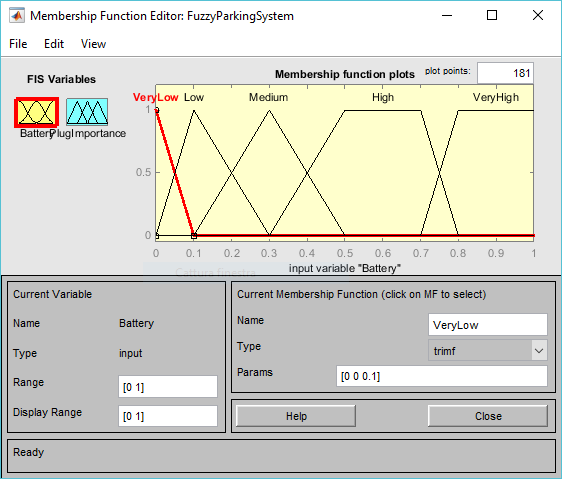
\includegraphics[width=1\textwidth]{img/Fuzzy/Battery.PNG}
		\caption{Input: Battery}
		\label{fig:subim1}
	\end{subfigure}
	\begin{subfigure}{.5\textwidth}
		\includegraphics[width=1\textwidth]{img/Fuzzy/PlugImportance.PNG}
		\caption{Output: PlugImportance}
		\label{fig:subim2}
	\end{subfigure}
	\begin{subfigure}{.5\textwidth}
		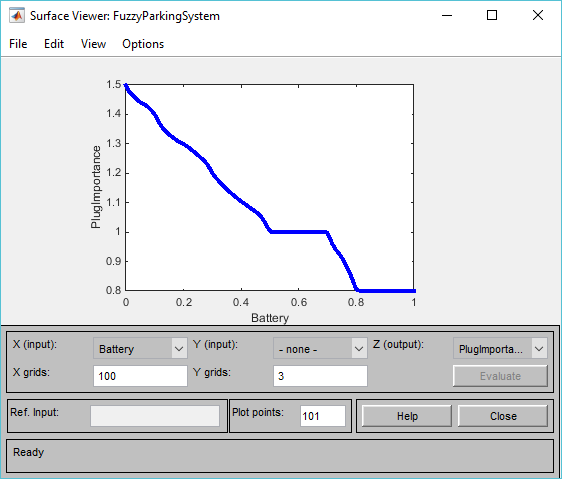
\includegraphics[width=1\textwidth]{img/Fuzzy/output.PNG}
		\caption{Function plane}
		\label{fig:subim3}
	\end{subfigure}
	
	\caption{Matlab plotting}
	\label{fig:image1}
\end{figure}